\documentclass{article}
\usepackage{graphicx}
\usepackage[utf8]{inputenc}
\usepackage{amsmath}
\usepackage{amssymb}
\usepackage{graphicx}
\usepackage{epstopdf}
\usepackage{inputenc}
\usepackage{latexsym}
\usepackage{setspace}
\usepackage{caption}
\usepackage{authblk}
\usepackage{float}
\setlength\parindent{24pt}
\usepackage[export]{adjustbox}


\begin{document}

\title{Digital data acquisition and analysis}
\author{Loïc James McKeever}
\affil{Mackenzie Levangie}

\maketitle

\section{Introduction}

The goal of this lab is to acquire and analyze digital data from an analog signal.  Specifically the data will be acquired from a function generator and the analysis will consist of plotting the signal and performing a FFT(Fast Fourier Transform) which will also be plotted so as to determine the frequency of the signal.  This will be done on a variety of different signals and a variety of different acquisition periods.  The data was acquired by connecting a function generator to a National Instruments data acquisition(DAQ) card and we wrote a code in Labwindows that allowed us to interface with the card.  We expect to accurately determine the frequency of various signals up to a certain cutoff(Nyquist frequency) and observe observe aliasing for signals above said cutoff. 

\section{Materials and Methods}

For the signal measured we used a function generator(GW Instek GFG-821 6A) connected to our computer using a National Instruments DAQ card(N114).  The code written in C in Labwindows would then acquire the data for a certain period of time at a certain rate which could be input by the user.  Once all the data has been acquired, with the press of a button, the code will analyze the data.
\\
The analysis of the data consists of several parts.  The first part is simply plotting the data on a 2-D plot, amplitude with respect to time.  This allows the user to visualize the signal being received.  The second part consists of calculating the power series of the data.  Specifically the function we used takes the Fast Fourier Transform(FFT) of the data, multiplies it by the complex conjugate of the FFT and divides it by the number of data points.  This function also gives us a frequency interval which we use to convert the time axis into a frequency axis.  Finally the Fourier transformed data is plotted with respect to frequency.  It is sometimes hard to determine the exact position of the peak visually though so the code will also determine the maximum value of the power series data, plot a line on the graph and display the exact frequency value of the peak on the user interface panel.  
\\
Finally the code also allows the user to save both data sets, the original data and the transformed data, to two text files.  The user can specify a name for the data and the files will be saved and the code will automatically specify in their titles whether it's the original data or the modified data.  This raw data was then analyzed using Excel.

\section{Results}

We started by setting the amplitude of the function generator to a 1 V, 100 Hz, sine wave.  We then acquired the data from the signal for a period of 10 ms at a sampling frequency of 1kHz(1000 points every second).  The data was plotted and the power spectrum was computed and plotted as well, see Figure 1.  The frequency was determined to be 78.99 Hz.

\begin{figure}[H]
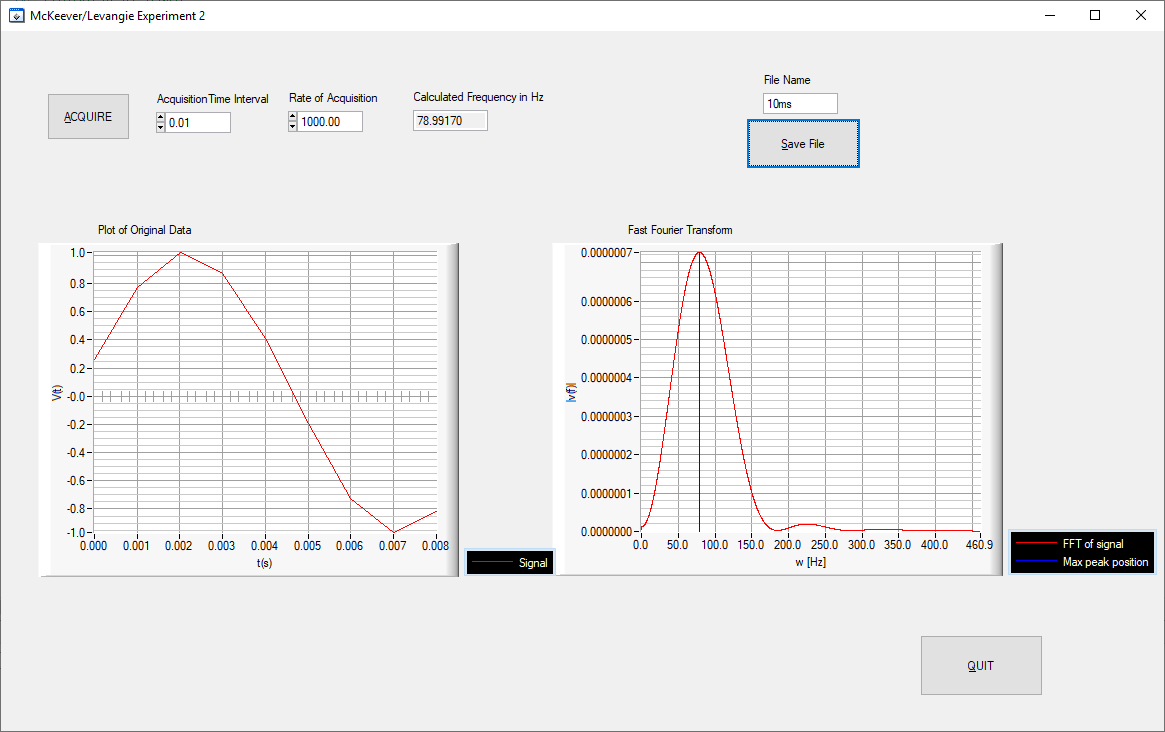
\includegraphics[scale=0.5,center]{Sine10ms.png}
\caption{This figure shows the plots of the original data and transformed data of a 100 Hz sine wave with an amplitude of 1 V sampled for 10 ms at a rate of 1 kHz.  The panel also displays the measured frequency which was 78.99 Hz.}
\end{figure}

The data was then saved and plotted in Excel, see Figures 2 and 3.  In Excel we were able to calculate the Full Width at Half Maximum(FWHM) of the peak in the power spectrum graph(see Figure 3) and it was found to be 84.41 Hz.  The FWHM is used to quantify the "sharpness" of the peak.  The smaller the FWHM the sharper the peak and the more accurate the result.

\begin{figure}[H]
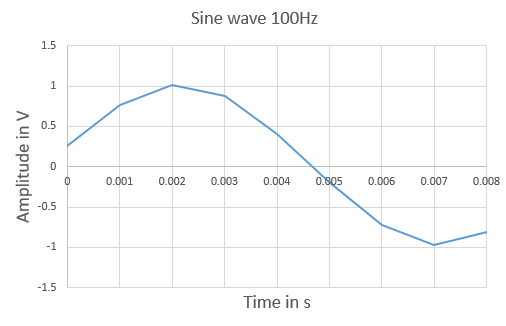
\includegraphics[scale=.6,center]{Sine10msex.PNG}
\caption{This figure shows the plot of the original 100 Hz sine wave signal sampled for 10 ms at a rate of 1 kHz.}
\end{figure}

\begin{figure}[H]
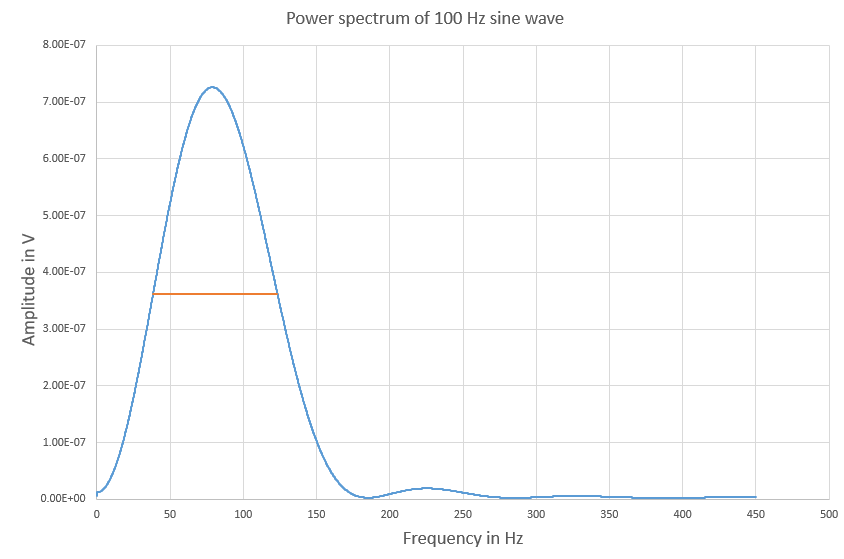
\includegraphics[scale=0.55,center]{Fouriersine10ms.PNG}
\caption{This figure shows the transformed data of 100Hz sine wave sampled for 10 ms at a rate of 1kHz.  The plot also shows the FWHM for the peak which is 84.81 Hz.}
\end{figure}

This was repeated using the same 100 Hz sine wave and the same 1 kHz sampling rate but we increased the sampling period to 50 ms(see Figures 4), the frequency was determined to be 100.71 Hz, and then again to 100 ms(see Figures 7), the frequency was determined to be 100.34 Hz.  The data for these graphs was also plotted in Excel, see Figures 5 and 6 for the 50 ms sampling period and Figures 8 and 9 for the 100 ms sampling period.  The FWHM was 17.64 Hz and 8.85 Hz for the sampling times of 50 ms and 100 ms respectively.

\begin{figure}[H]
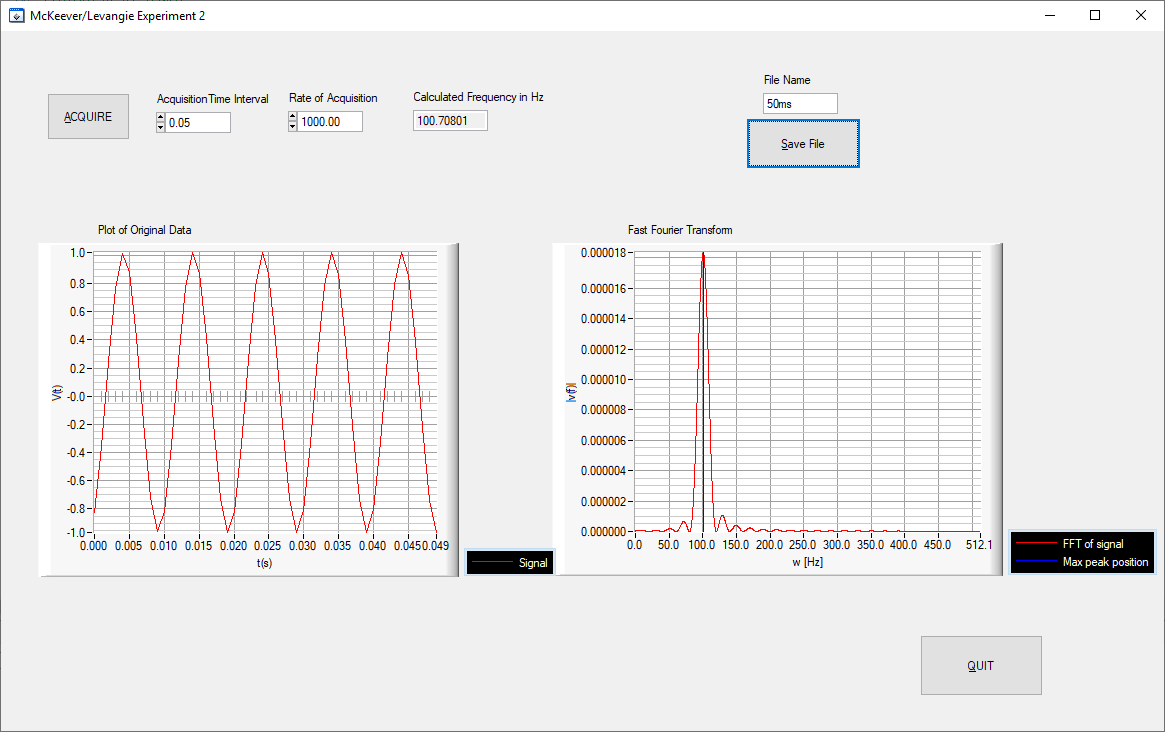
\includegraphics[scale=0.5,center]{Sine50ms.png}
\caption{This figure shows the plots of the original data and transformed data of 100 Hz sine wave with an amplitude of 1 V sampled for 50 ms at a rate of 1 kHz.  The panel also displays the measured frequency which was 100.71 Hz.  This is only 0.71 Hz different than what we'd expect which is much better than when we only sampled for 10 ms.}
\end{figure}

\begin{figure}[H]
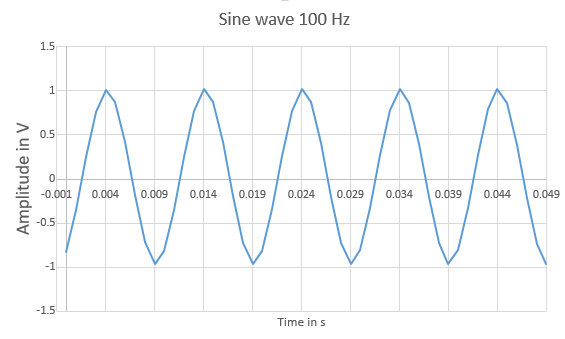
\includegraphics[scale=.75,center]{Sine50msex.PNG}
\caption{This figure shows the plot of the original 100 Hz sine wave signal sampled for 50 ms at a rate of 1 kHz.}
\end{figure}

\begin{figure}[H]
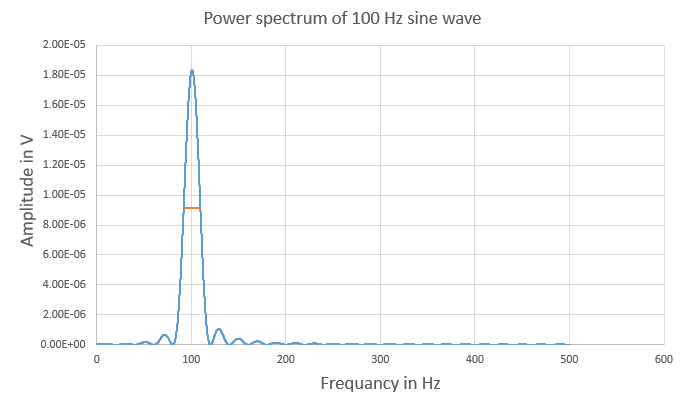
\includegraphics[scale=0.75,center]{Fouriersine50ms.PNG}
\caption{This figure shows the transformed data of 100Hz sine wave sampled for 50 ms at a rate of 1kHz.  The plot also shows the FWHM for the peak which is 17.64 Hz which is much smaller than the FWHM for the data sampled for 10 ms.  }
\end{figure}

\newpage

\begin{figure}[H]
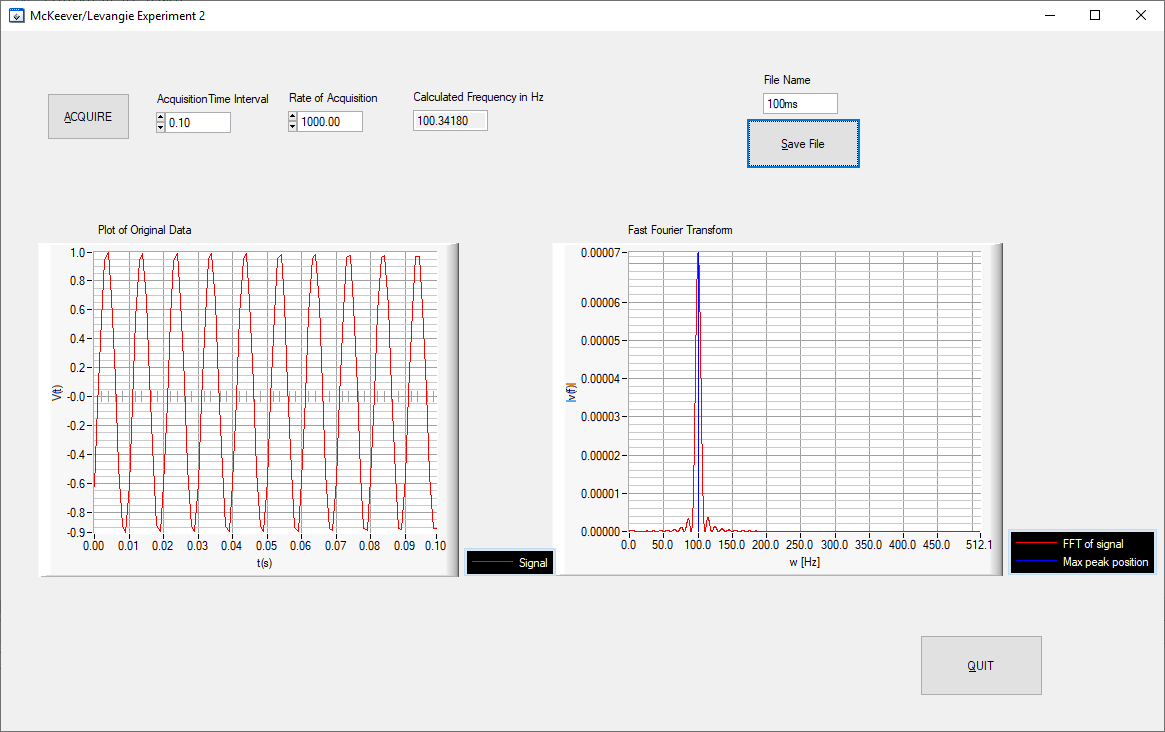
\includegraphics[scale=0.5,center]{Sine100ms.png}
\caption{This figure shows the plots of the original data and transformed data of a 100 Hz sine wave with an amplitude of 1 V sampled for 100 ms at a rate of 1 kHz.  The panel also displays the measured frequency which was 100.34 Hz.}
\end{figure}

\begin{figure}[H]
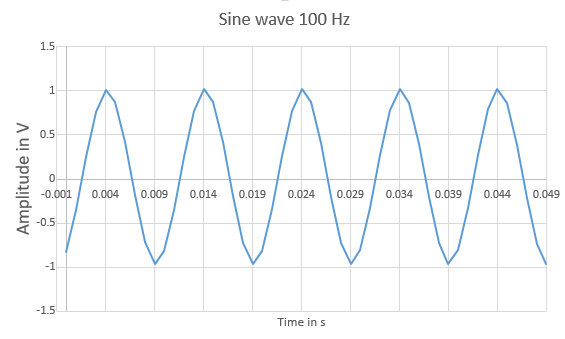
\includegraphics[scale=.6,center]{Sine50msex.PNG}
\caption{This figure shows the plot of the original 100 Hz sine wave signal sampled for 100 ms at a rate of 1 kHz.}
\end{figure}

\begin{figure}[H]
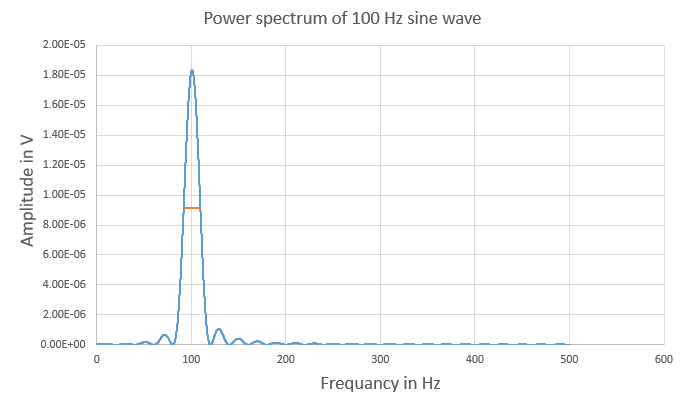
\includegraphics[scale=0.55, center]{Fouriersine50ms.PNG}
\caption{This figure shows the transformed data of 100Hz sine wave sampled for 50 ms at a rate of 1kHz.  The plot also shows the FWHM for the peak which is 8.85 Hz which is about half than the FWHM for the data sampled for 50 ms.}
\end{figure}

Figures 10 through 12 show the same process with a triangle wave(without saving the data) and figures 13 through 15 plot and analyze data from a square wave.

\begin{figure}[H]
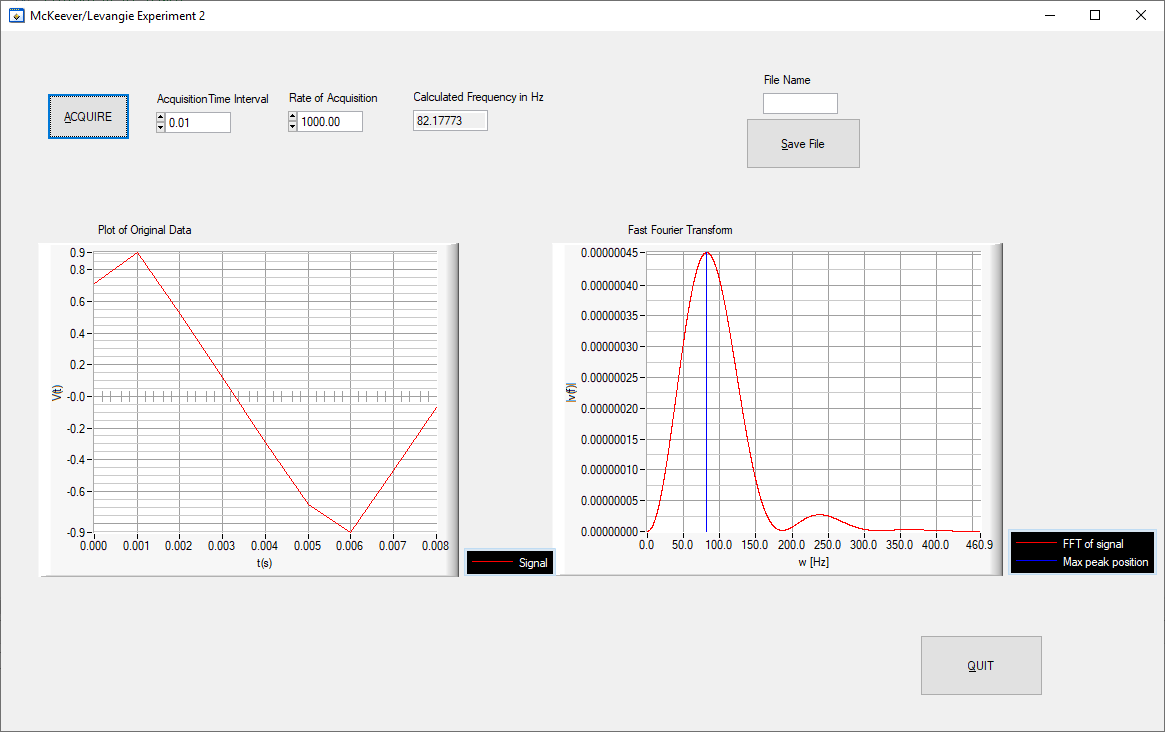
\includegraphics[scale=0.4,center]{Triangle10ms.png}
\caption{This figure shows the plots of the original data and transformed data of a 100 Hz triangle wave with an amplitude of 1 V sampled for 10 ms at a rate of 1 kHz.  The panel also displays the measured frequency which was 82.18 Hz.}
\end{figure}

\begin{figure}[H]
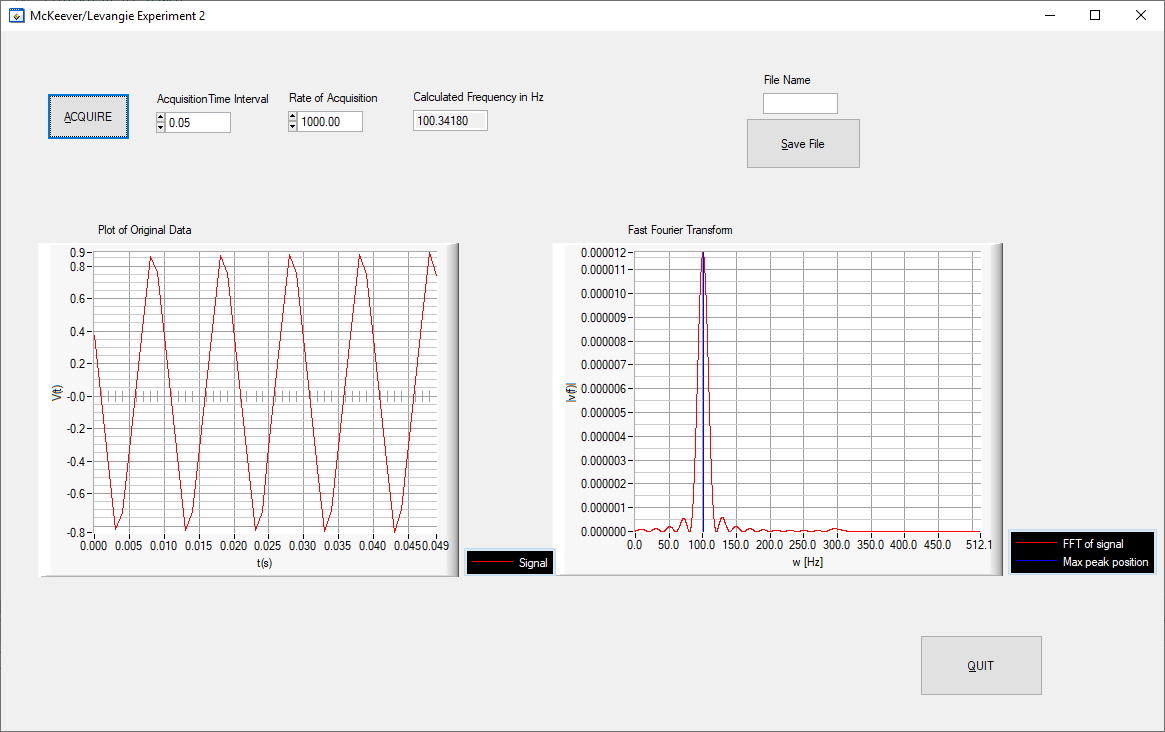
\includegraphics[scale=0.4,center]{Triangle50ms.png}
\caption{This figure shows the plots of the original data and transformed data of a 100 Hz triangle wave with an amplitude of 1 V sampled for 50 ms at a rate of 1 kHz.  The panel also displays the measured frequency which was 100.34 Hz.}
\end{figure}

\begin{figure}[H]
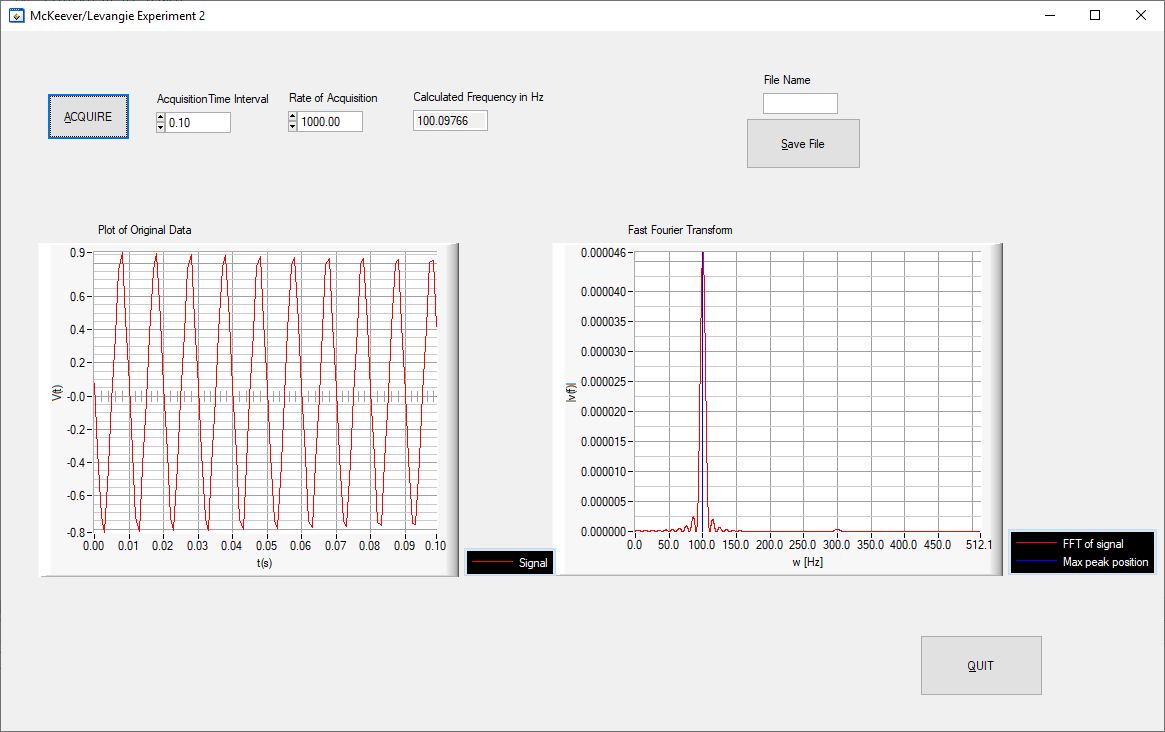
\includegraphics[scale=0.4,center]{Triangle100ms.png}
\caption{This figure shows the plots of the original data and transformed data of a 100 Hz triangle wave with an amplitude of 1 V sampled for 100 ms at a rate of 1 kHz.  The panel also displays the measured frequency which was 100.10 Hz.}
\end{figure}


\begin{figure}[H]
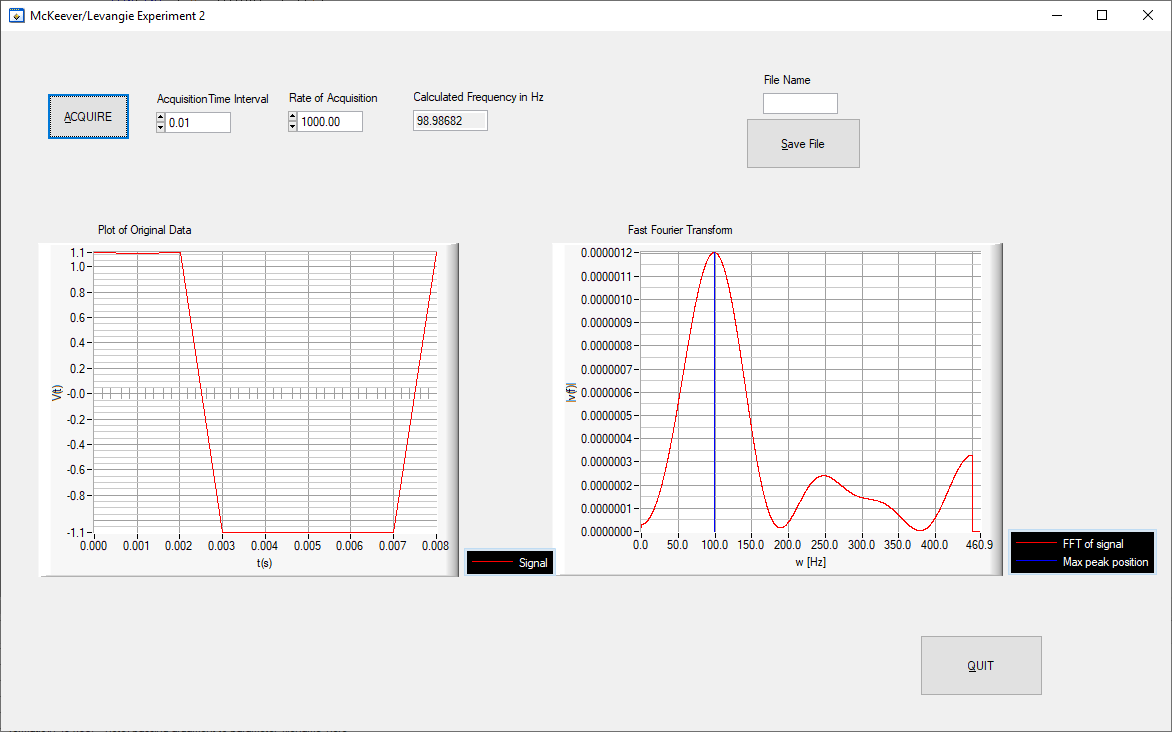
\includegraphics[scale=0.39,center]{Square10ms.png}
\caption{This figure shows the plots of the original data and transformed data of a 100 Hz square wave with an amplitude of 1 V sampled for 10 ms at a rate of 1 kHz.  The panel also displays the measured frequency which was 98.91 Hz.}
\end{figure}


\begin{figure}[H]
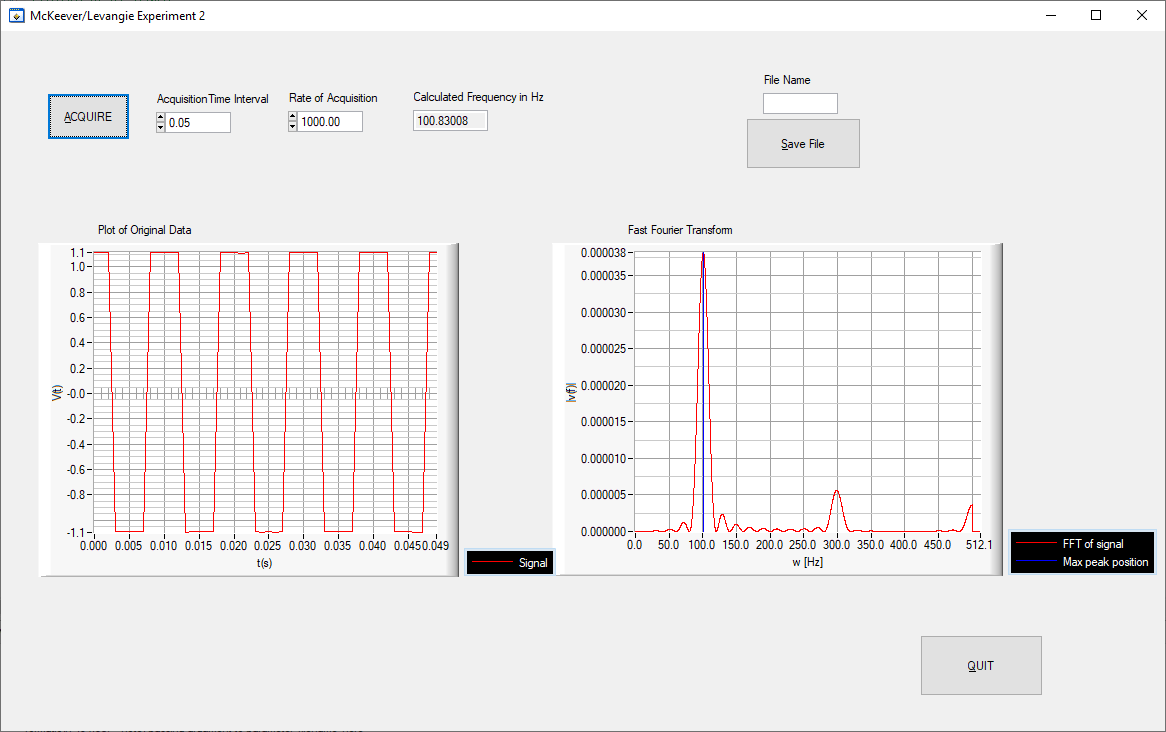
\includegraphics[scale=0.39,center]{Square50ms.png}
\caption{This figure shows the plots of the original data and transformed data of a 100Hz square wave with an amplitude of 1 V sampled for 50 ms at a rate of 1 kHz.  The panel also displays the measured frequency which was 100.83 Hz.}
\end{figure}


\begin{figure}[H]
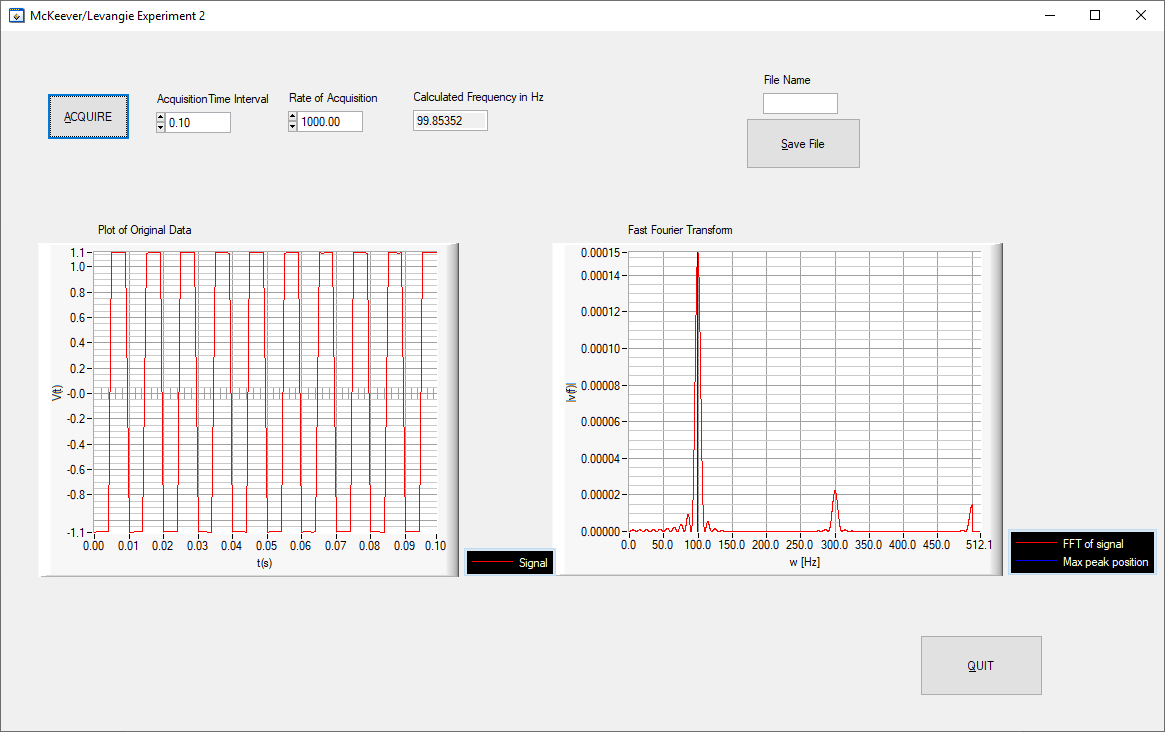
\includegraphics[scale=0.4,center]{Square100ms.png}
\caption{This figure shows the plots of the original data and transformed data of a 100 Hz square wave with an amplitude of 1 V sampled for 100 ms at a rate of 1 kHz.  The panel also displays the measured frequency which was 99.85 Hz.}
\end{figure}

The Nyquist frequency is the maximum frequency that can be determined from data taken at a certain sampling rate.  It is determined by the following equation;
$$f_{Nyquist}=\frac{1}{2\tau}=\frac{f_{sampling}}{2}$$ where $\tau$ is the time between sampled data points and is one over the sampling frequency $f_{sampling}$.

Here we used a sampling frequency of 1 kHz so our Nyquist frequency will be 500 Hz.  We then attempted to plot and transform the data from a signal at the Nyquist frequency(see Figures 16, 17 and 18), at one and a half times the Nyquist frequency(see Figures 19,20 and 21) and finally at twice the Nyquist frequency(see Figures 22, 23 and 24).

\begin{figure}[H]
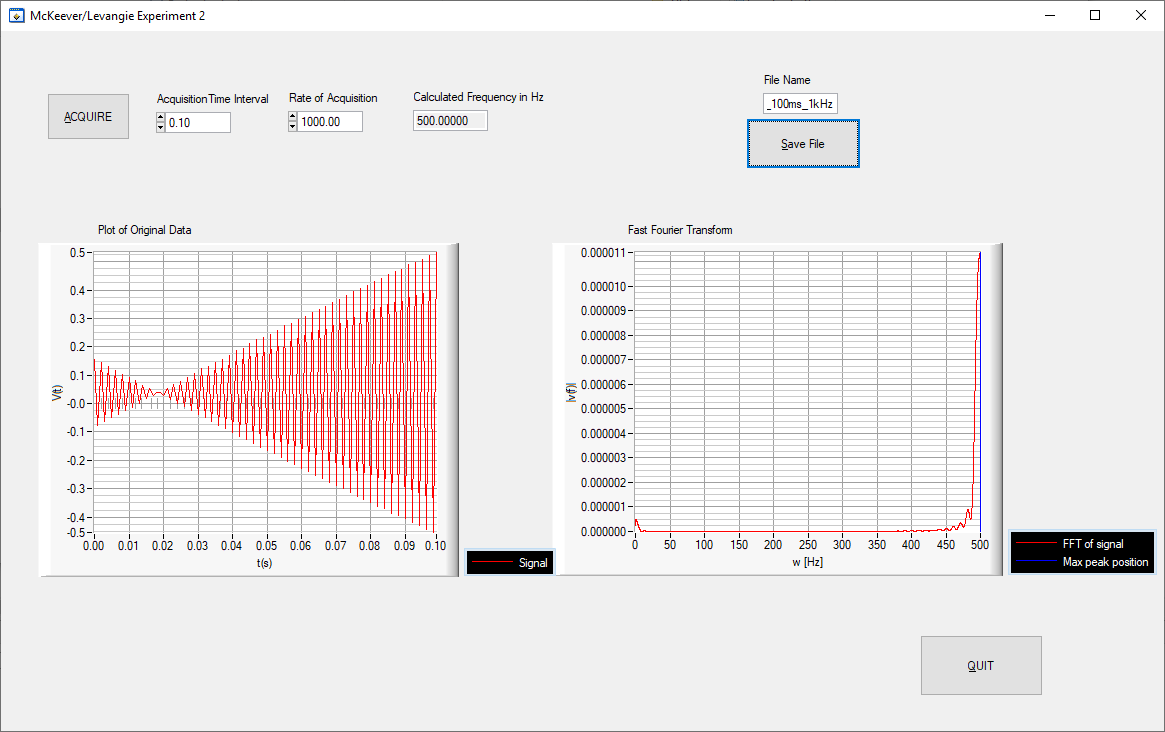
\includegraphics[scale=0.4,center]{Nyquist.png}
\caption{This figure shows the plots of the original data and transformed data of a 500 Hz sine wave with an amplitude of 1 V sampled for 100 ms at a rate of 1 kHz.  The panel also displays the measured frequency which was 500 Hz.}
\end{figure}

\begin{figure}[H]
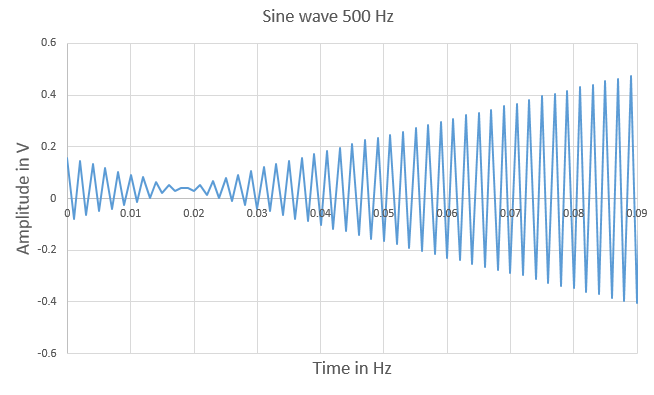
\includegraphics[scale=0.7,center]{SignalNyquist.PNG}
\caption{This figure shows the plot of the original 500 Hz sine wave signal sampled for 100 ms at a rate of 1 kHz.}
\end{figure}

\begin{figure}[H]
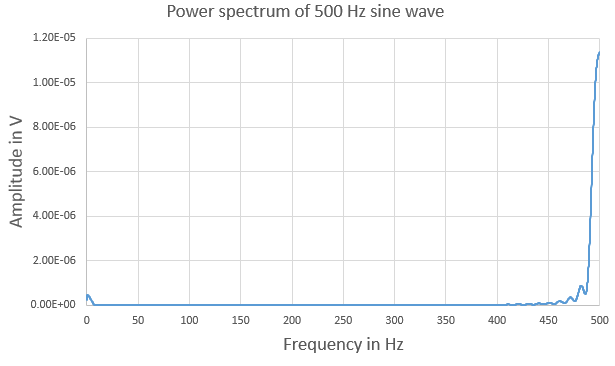
\includegraphics[scale=0.7,center]{FourierNyquist.PNG}
\caption{This figure shows the transformed data of 500 Hz sine wave sampled for 100 ms at a rate of 1kHz.}
\end{figure}

\begin{figure}[H]
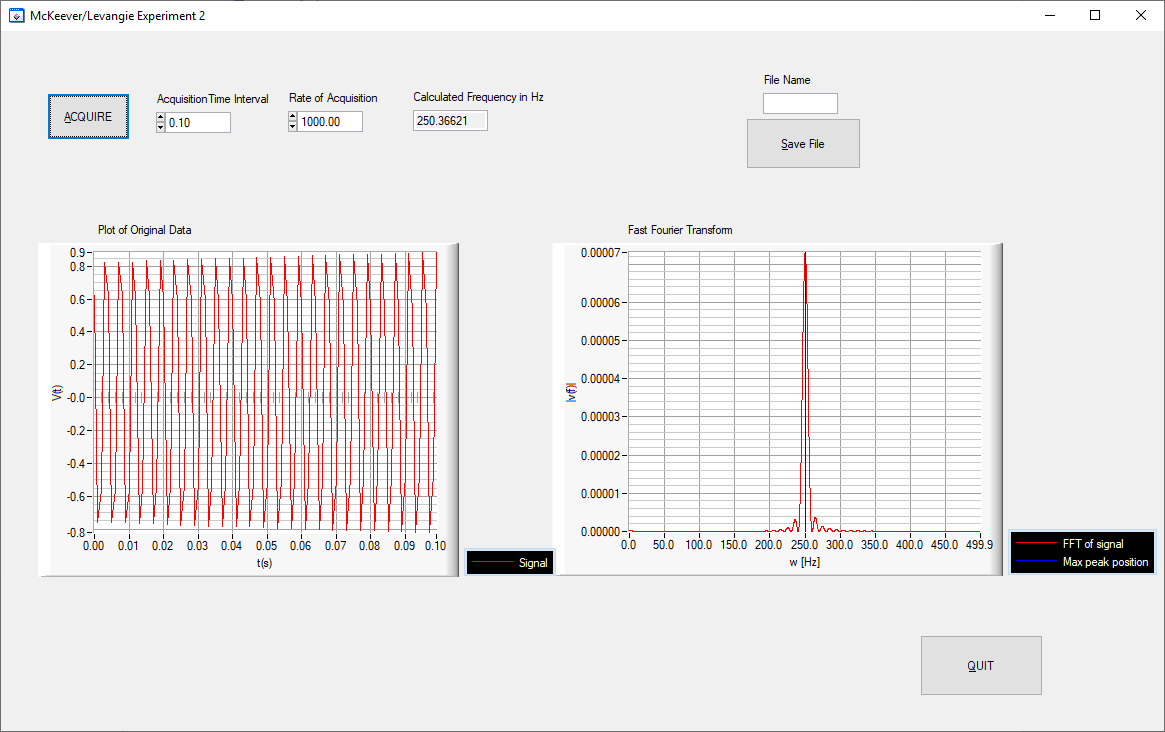
\includegraphics[scale=0.4,center]{Nyquist+750.png}
\caption{This figure shows the plots of the original data and transformed data of a 750 Hz sine wave with an amplitude of 1 V sampled for 100 ms at a rate of 1 kHz.  The panel also displays the measured frequency which was 250.37 Hz.}
\end{figure}

\begin{figure}[H]
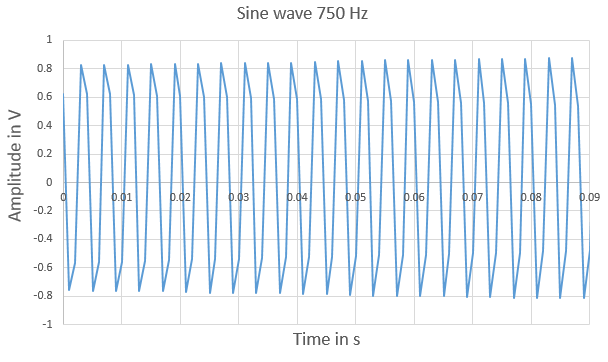
\includegraphics[scale=0.7,center]{Signal750.PNG}
\caption{This figure shows the plot of the original 750 Hz sine wave signal sampled for 100 ms at a rate of 1 kHz.}
\end{figure}

\begin{figure}[H]
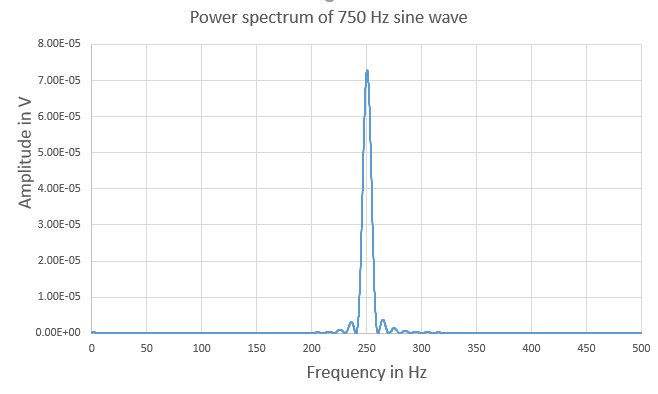
\includegraphics[scale=0.7,center]{Fourier750.PNG}
\caption{This figure shows the transformed data of 750 Hz sine wave sampled for 100 ms at a rate of 1kHz.}
\end{figure}

\begin{figure}[H]
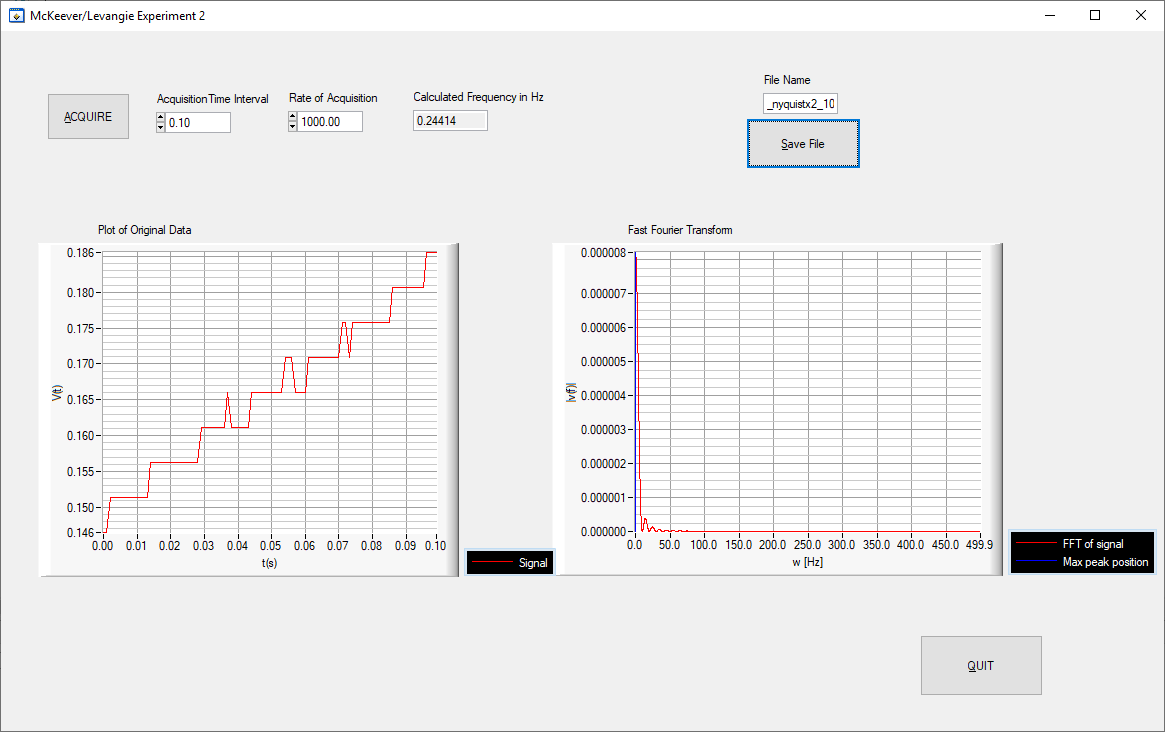
\includegraphics[scale=0.4,center]{2xNyquist.png}
\caption{This figure shows the plots of the original data and transformed data of 1 kHz square wave with an amplitude of 1 V sampled for 100 ms at a rate of 1 kHz.  The panel also displays the measured frequency which was 0.24 Hz.}
\end{figure}

\begin{figure}[H]
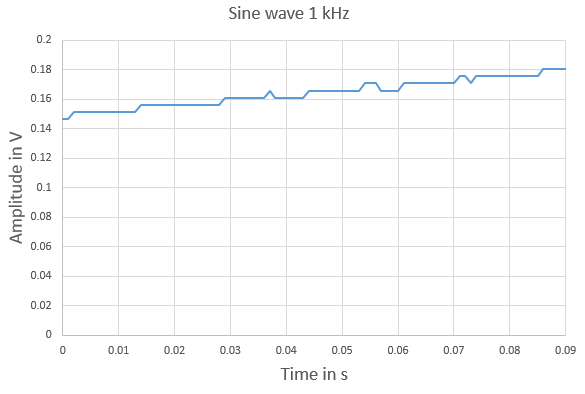
\includegraphics[scale=0.7,center]{Signal2xNyquist.PNG}
\caption{This figure shows the plot of the original 1 kHz sine wave signal sampled for 100 ms at a rate of 1 kHz.}
\end{figure}

\begin{figure}[H]
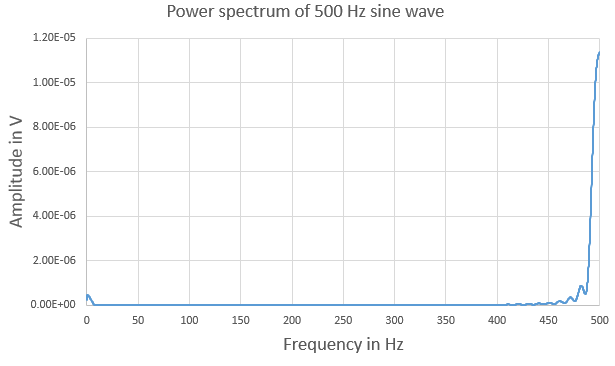
\includegraphics[scale=0.7,center]{FourierNyquist.PNG}
\caption{This figure shows the transformed data of 1 kHz sine wave sampled for 100 ms at a rate of 1kHz.}
\end{figure}

\section{Discussion}

We can see on the graph on the left in Figure 1 that the signal is not very smooth due to the relatively small amount of points taken(9 points).  We can also see that the peak in the power spectrum plot is very wide.  It should also be noted that the measured frequency, 79 Hz, is 21 Hz less than the expected value, 100 Hz.  This is due to low sampling frequency.
 
The graph in Figure 4 shows that the signal still doesn't look very smooth because the sampling rate hasn't changed but we can see that the peak of the power spectrum is much sharper and the measurement of the signal's frequency is much more accurate.  This tells us that the sampling frequency is less important when it comes to getting an accurate result than the sampling period is.

When the sampling period was increased again to 100 ms the measured frequency at 100.34 Hz 100  was again closer to the expected value of 100 Hz as we can see in Figure 7.  The FWHM also went down to 8.85 Hz from 17.64 Hz.  It now becomes a trade off;  a larger sampling time will guarantee more accurate results but if they're only slightly more accurate it might not be worth the increase in time, for both the acquisition and the computing time of the code, required. 

The results for the triangle and square waves were very similar to those of the sine wave; inaccurate observed frequency at low sampling periods and increased accuracy at higher sampling frequencies.  The difference that should be noted though is the secondary and tertiary(in the case of the square wave) peaks.  For the triangle wave there is a small peak at 300 Hz, best seen in Figure 12,  and for the square wave there are more substantial peaks at 300 and 500 Hz, best seen in Figure 15.  This is exactly what we'd expect if our program was working correctly.  This comes from the fact that neither of them are pure sine waves.  They can be approximated as a sum of sine waves so when they undergo FFT we can see exactly their exact composition in terms of sine waves with different frequencies.  

The sampling frequency might not be as important as the sampling period when it comes to accurately determining the frequency of a signal but it is vitally important when it comes to the range of signals that can be analyzed correctly.  We were able to accurately determine the frequency at the Nyquist frequency(500 Hz) but there was a loss of amplitude in the signal as we can see in Figure 17, the amplitude should be 1 V at each oscillation but the maximum and minimums seem to vary linearly with time.  This is expected and is due to aliasing.  Aliasing is due to the fact that at too low a sampling frequency information about the signal is lost in between the time each data point is taken.  At one and a half times the Nyquist frequency the measured frequency was completely inaccurate and there was a loss of amplitude again, see Figure 19.  Same can be said for the signal at twice the Nyquist frequency, see Figure 22, although the original signal is completely lost and doesn't even look like a sine wave anymore.  This is consistent with what we'd expect from sampling a signal larger than the Nyquist frequency.  The observed frequency is given by;
$$f_{observed}=|f_{signal}-f_{sampling}|$$
So for an signal frequency of 750 Hz we should get an observed frequency of 250 Hz and as we can see in Figure 19 we found 250.36 Hz as expected.
Should we want to sample these larger frequencies we'd need to increase the sampling frequency.   


\section{Conclusions}

In conclusion, our code allowed us to accurately measure the frequency of 100 Hz signals in the form of sine, triangle and square waves.  We observed their frequencies to be 100.34 Hz, 100.10 Hz and 99.85 Hz respectively.  We also determined that the largest factor for getting an accurate result is sampling period.  The data was sampled at 10ms, 50ms and 100ms and the FWHM of our power spectrum peaks were 84.81 Hz, 17.64 Hz and 8.85 Hz respectively.  In terms what frequency range that could be accurately measured we learned that the sampling frequency was most important.  When the input frequency was larger than Nyquist frequency(half the sampling frequency and 500 Hz in our case)  the observed frequency was much lower than actual input frequency which was expected.  When we measured a 750 Hz signal we observed a frequency of 250.37Hz and when we measured a 1 kHz signal the observed frequency was only 0.24 Hz.  Based on the theory we expected frequencies of 250 Hz and 0 Hz respectively. 

\section{Appendix}

See code attached.

\end{document}
